
\subsection{Теоремы о продолжении решения для нормальной системы дифференциальных уравнений}

Теоремы Коши носят существенно локальный характер. Решение и единственность задачи Коши будет существовать на отрезке Пеано. Теперь сделаем отход от единственности и докажем, чтo $\Vec{\varphi}(t)$ и $\Vec{\psi}(t)$ есть решение задачи Коши, то они будут совпадать на промежутке, где они оба определены (отход от локальности).

%% (1) и (2) опредленно в пред части билета
\begin{theorem}
	Пусть $\Vec{\varphi}(t)$ решение $\eqref{equ:norm-sys} \wedge \eqref{equ:init-cond}$ определенно на $\langle a, b \rangle$, a  $\Vec{\psi}(t)$ решение $\eqref{equ:norm-sys} \wedge \eqref{equ:init-cond}$ определенно на $\langle c, d \rangle$.
	Тогда $\Vec{\varphi}(t) \equiv \Vec{\psi}(t)$ на $\langle r_1, r_2 \rangle = \langle a, b \rangle \cap \langle c, d \rangle$.
\end{theorem}
\begin{proof}
	От противного: $\exists t^* \in \langle r_1, r_2 \rangle$, где $\Vec{\varphi}(t^*) \neq \Vec{\psi}(t^*)$, тогда $t^* \neq t_0$ и предположим, что $t^* > t_0$. 
	Рассмотрим множество $N$ точек такое, что $t \in [t_0, t^*]$ и $\Vec{\varphi}(t) = \Vec{\psi}(t)$. \\
	Покажем, что \underline{множество замкнуто}: \\
	Рассмотрим сходящуюся послед-сть $t_1 \ldots t_n \in N$, $\displaystyle \lim_{n\to\infty} t_n = \overline{t}$. Нужно показать, что $\overline{t} \in N$:\\
	Рассмотрим $\displaystyle \lim_{n\to\infty} \Vec{\varphi}(t_n) = \lim_{n\to\infty} \Vec{\psi}(t_n)$ (равны по выбору множества $N$). И из непрерывности выбранных функций получаем, что $\displaystyle \lim_{n\to\infty} \Vec{\varphi}(t_n) = \lim_{n\to\infty} \Vec{\psi}(t_n) = \Vec{\varphi}(\overline{t}) = \Vec{\psi}(\overline{t})$ $\Rightarrow$ замкнутость. \\
	Из замкнутости и ограниченности мн-ва $N$ $\Rightarrow$ $\exists \widetilde{t} = sup\ N$, $\widetilde{t} \in N$. Очевидно, что $\widetilde{t} < t^* < r_2$.
	
	Пусть $\Vec{\varphi}(\widetilde{t}) = \Vec{\psi}(\widetilde{t}) = \vec{y_0}.$ Поставим задачу Коши в $t = \widetilde{t}$. По основной теореме на $[\widetilde{t} - \widetilde{h}; \widetilde{t} + \widetilde{h}]$ решения $\vec{\psi}(t)$ и $\vec{\varphi}(t)$ совпадают, что противоречит тому факту, что $\widetilde{t} = \sup N$ $\Rightarrow  \vec{\varphi} (t^*) = \vec{\psi}(t^*)$, а значит и $\vec{\varphi} = \vec{\psi}$ на всём $\langle r_1; r_2\rangle$. Аналогичные рассуждения для $t^* < t_0$. 
\end{proof}

\begin{definition} 
	$\Vec{\varphi}(t)$ определена на $\langle a, b\rangle$ и решение $\eqref{equ:norm-sys} \wedge \eqref{equ:init-cond}$, если $\exists \Vec{\psi}(t)$ на $\langle a, b_1\rangle \supset \langle a, b\rangle$, и решение $\eqref{equ:norm-sys} \wedge \eqref{equ:init-cond}$ и $\Vec{\varphi}(t) \equiv \Vec{\psi}(t)$ на $\langle a, b\rangle$, тогда $\Vec{\varphi}(t)$ называется продолжаемым вправо, а $\Vec{\psi}(t)$ продолжением решения $\Vec{\varphi}(t)$ задачи Коши
\end{definition}

\begin{definition} 
	Решение, которое нельзя продолжить ни вправо, ни влево называется непродолжаемым решением
\end{definition}

\begin{remark}
	По сути данная теорема является усилением задачи Коши. Вместо отрезка Пеано мы получили, что решение задачи Коши может быть продолжено на промежуток, где они оба определены.
\end{remark}

\begin{theorem}
	Пусть имеется задача Коши $\eqref{equ:norm-sys} \wedge \eqref{equ:init-cond}$ и $\vec{f}(t, \vec{x}), \dfrac{\partial f^i}{\partial x_j}, i, j = \overline{1, n}$ непрерывны в $\Omega \subset \mathbb{R}^{n+1}$. Тогда $\forall (t_0, \vec{x_0}) \in \Omega \ \exists!$ непродолжаемое решение задачи $\eqref{equ:norm-sys} \wedge \eqref{equ:init-cond}$.
\end{theorem}
\begin{proof}
	Рассмотрим множество решений задач Коши $\eqref{equ:norm-sys} \wedge \eqref{equ:init-cond}$. Каждое решение задачи определенно на промежутке $\langle R_1, R_2 \rangle$, тогда пусть $T_1 = inf\ R_1, T_2 = sup\ R_2$. Построим решение $\vec{\varphi}(t)$ задачи $\eqref{equ:norm-sys} \wedge \eqref{equ:init-cond}$ на $(T_1, T_2)$:\\
	Выберем $t^* > t_0$, тогда $\exists\ \vec{\psi}(t)$, чей промежуток содержит $t^*$ (в силу выбора промежутка $(T_1, T_2)$). Положим $\vec{\varphi}(t^*) \defeq \vec{\psi}(t^*)$. Покажем, что значение $\vec{\varphi}(t^*)$ не зависит от выбора $\vec{\psi}(t)$:\\
	Пусть $\displaystyle \vec{\hat{\psi}}(t)$ другое решение задачи Коши $\eqref{equ:norm-sys} \wedge \eqref{equ:init-cond}$ содержащее $t^*$. Из теоремы сущ. и единст. решения задачи Коши следует, что решения будут совпадать на промежутке, где они оба определены. Т.к. $t^*$ принадлежит этому промежутку, то $\vec{\hat{\psi}}(t^*) = \vec{\psi}(t^*)$.\\ 
	Построение вниз проводится аналогично. Итак, $\vec{\varphi}(t)$ решение $\eqref{equ:norm-sys} \wedge \eqref{equ:init-cond}$ на $T_1 < t < T_2$. Это решение \underline{является продолжением любого из множества решений} задачи Коши. Допустим, $\vec{\widetilde{\varphi}}(t)$ решение $\eqref{equ:norm-sys} \wedge \eqref{equ:init-cond}$ на $r_1 \leq t \leq r_2$ и $T_1 \leq r_1 \leq r_2 \leq T_2$ $\Rightarrow$ $\vec{\widetilde{\varphi}}(t) = \vec{\varphi}(t)$ ($\vec{\varphi}(t)$ продолжение решения по доказанной выше теореме). \\Покажем, что $\vec{\varphi}(t)$ является \underline{непродолжаемым решением} $\eqref{equ:norm-sys} \wedge \eqref{equ:init-cond}$:
	Допустим, что имеется ещё  одно решение $\vec{\chi}(t)$, определённое на $(\gamma_1; \gamma_2)$ и оно является продолжением $\vec{\varphi}(t)$. Тогда, либо $\gamma_1 < T_1$, либо $\gamma_2 > T_2$, что невозможно, т.к. $T_1 = inf\ R_1, T_2 = sup\ R_2$ по построению. \\
	Покажем, что непродолжаемое решение $\vec{\varphi}(t)$ является \underline{единственным}:\\
	От противного, пусть $\exists$ $\vec{\varphi}(t)$ непродолжаемое решение на $(T_1, T_2)$ и $\vec{\psi}(t)$ на $(\widetilde{T_1}, \widetilde{T_2})$. Для определённости $\widetilde{T_1} < T_1$, тогда рассмотрим такое решение
	$\vec{\chi}(t)$ = 
	$\left[ 
		\begin{gathered} 
			\vec{\psi}(t)\ \text{на}\ (\widetilde{T_1}, T_1), \\ 
			\vec{\varphi}(t)\ \text{на}\ (T_1, T_2); \\ 
		\end{gathered} 
	\right.$
	$\Rightarrow$ $\vec{\chi}(t)$  -- продолжение $\vec{\varphi}(t)$, противоречие. Аналогично строя остальные решения получаем, что $\vec{\varphi}(t) \equiv \vec{\psi}(t)$ 
\end{proof}

\begin{remark}
	В теореме не сказано, как определить $T_1$ и $T_2$. Если усилить условия теоремы, а именно $\Omega$ есть ограниченная область, то любое непродолжаемое решение выходит на границу этой области.\\
	Из этих утверждений следует, что если под интегральной кривой понимать график непродолжаемого решения, то через каждую точку $(x_0, y_0) \in \Omega$ проходит только одна кривая.
\end{remark}

\subsection{Непрерывная зависимость от параметров решения задачи Коши для нормальной системы ДУ}
	Рассматриваем уравнение
	\begin{equation}\label{init_2-5_tick}
	y' = f(x, y, \mu)
	\end{equation}
	с задачей Коши $y(x_0, \mu) = y_0$, где $\mu$ -- параметр.
\begin{theorem}
	Пусть $\mathcal{G}$ -- область в пр-ве $(x, y, \mu)$. Если ф-ции $f(x, y, \mu)$, $\dfrac{\partial f(x, y, \mu)}{\partial y}$ непрерывны в области по совокупности переменных и точка $(x_0, y_0, \mu_0) \in \mathcal{G}$, то решение задачи Коши (\ref{init_2-5_tick} $y(x, \mu)$) непрерывно по совокупности переменных $(x; \mu)$ в некоторой области $|x - x_0| \leq h, |\mu - \mu_0| \leq \delta$
\end{theorem}
\begin{proof}
	Аналогично доказательство основной теоремы \ref{ОсновнаяТеорема} сведем задачу Коши к эквивалентной её интегральному уравнению 
	\begin{equation}\label{eq_int_1}
		y(x, \mu) = y_0 + \int_{x_0}^{x} f(\tau, y(\tau, \mu)) d\tau,
	\end{equation}
	или в операторной форме:
	\begin{equation}\label{eq_int_2}
		y(x, \mu) = A(y(x, \mu)),
	\end{equation}
	где $\displaystyle A(y(x, \mu)) = y_0 + \int_{x_0}^{x} f(\tau, y(\tau, \mu)) d\tau$.\\
	Выберем параллелепипед $\prod = \{ |x - x_0| \leq a,\ |\mu - \mu_0| \leq \delta, |y - y_0| \leq b\}$, целиком лежащей в области $\mathcal{G}$. В силу условий теоремы $\displaystyle \exists\ K = \max_{\prod \ }|f(x, y, \mu)|,\ C = \max_{\prod \ } \left| \frac{\partial f(x, y, \mu)}{\partial y} \right|$.\\ 
	Применим к (\ref{eq_int_2}) принцим сжатых отображений. В качестве $B$ возьмём пр-во ф-ций $y(x, \mu)$ непрерывных в прямоугольнике $\{|x - x_0| \leq h,\ |\mu - \mu_0| \leq \delta\}$, где $h > 0$ будет выбрано с нормой $\displaystyle||y(x, \mu)||_C = \max_{|x - x_0| \leq h\ } |y (\mu, x)|$. В качестве $M \subset B$ возьмём множество функций из $B$ таких, что $||y(x, \mu) - y_0||_C \leq b$.\\
	1) Нужно, чтобы $A(y(x, \mu)) \in M$, если $y(x, \mu) \in M$. $||A(y) - y_0|| = \left|\left|\displaystyle \int_{x_0}^{x} f(\tau, y(\tau, \mu)) d\tau \right|\right| \leq \displaystyle \left|\int_{x_0}^{x} f(\tau, y(\tau, \mu)) d\tau\right| \leq K \cdot h\ \Rightarrow$ Необходимо, чтобы $K\cdot h \leq b\ \Rightarrow h = min\ \{a, \frac{b}{K}\}$. \\
	2) Нужно, чтобы $A_x$ было сжатием, т.\ е.\ $||A\varphi - A\psi|| \leq k \cdot ||\varphi - \psi||,\ 0 < k < 1$. \\
	$$||A\varphi - A\psi|| = \left|\left|\displaystyle\int_{x_0}^{x} \Big( f(\tau, \varphi(\tau, \mu)) - f(\tau, \psi(\tau, \mu)) \Big) \cdot d\tau \right|\right| \leq $$
	$$ \leq \left|\displaystyle \int_{x_0}^{x} ||f(\tau, \varphi(\tau, \mu)) - f(\tau, \psi(\tau, \mu))|| \cdot d\tau \right| \leq $$ 
	$$ \leq \text{(По лемме Адамара)} \leq C\cdot h\cdot 1\cdot ||\varphi - \psi||\ \Rightarrow$$
	Необходимо, чтобы $C\cdot h < 1\ \Rightarrow h < \dfrac{1}{C}$.
	Т.\ е. при 
	$\begin{cases} 
		h \leq min ~ \left \{a, \frac{b}{K} \right \}, \\
		h < \dfrac{1}{C}. 
	\end{cases}$
	оператор $A$ является сжатием и обладает единственным решением операторного уравнения $y(x, \mu) = A(y(x, \mu))$, а значит и задача Коши (\ref{init_2-5_tick}). Причём решение $y(x, \mu)$ непрерывно по совокупности переменных.
\end{proof}
\subsection{Дифференцируемость решения по параметру}
	Пусть $y(x, \mu)$ является решением задачи Коши (\ref{init_2-5_tick}). Введем функцию $z(x, \mu)$:\ $z(x, \mu) = \dfrac{\partial y(x, \mu)}{\partial \mu}$
\begin{theorem}
	Если $f(x, y, \mu)$ как функция трёх переменных в области $\mathcal{G}$ пр-ва $(x, y, \mu)$ $p$ раз непрерывно дифференцируема по $(y, \mu)$ и $p - 1$ раз непрерывно дифференцируема по $x$, тогда решение задачи Коши (\ref{init_2-5_tick}) $y(x, \mu)$ является $p$ раз непрерывно дифференцируема по совокупности $(x, \mu)$.
\end{theorem}
\begin{proof}
	В 15 лекции от 10.12.20 года лектор сказал, что доказывать не будет . Запись текущего года на ютубе отсутствует. В Федорюке проводится доказательство для $p = 1$ (см следствие).
\end{proof}

\begin{corollary}
	$\dfrac{\partial}{\partial \mu} \Big(\dfrac{dy}{dx}\Big) = \dfrac{\partial}{\partial \mu} \Big(f(x, y(x, \mu), \mu)\Big) = \dfrac{\partial f}{\partial y} \cdot \dfrac{\partial y}{\partial \mu} + \dfrac{\partial f}{\partial \mu}$\\
	С задачей Коши: $\dfrac{\partial z}{\partial \mu}(x_0) = \dfrac{\partial y_0}{\partial \mu} \Rightarrow$ \\
	$\Rightarrow \dfrac{d}{dx} \Big( \dfrac{\partial y}{\partial \mu} \Big) = $ \fbox{$z_x' = \dfrac{\partial f}{\partial y} \cdot z + \dfrac{\partial f}{\partial \mu}$} $- ~ \text{уравнение в вариациях для} ~ (\ref{init_2-5_tick})$.
\end{corollary}

\begin{remark}
	Уравнение в вариациях всегда линейное.
\end{remark}

\subsection{Задача Коши для уравнения первого порядка, не разрешенного относительно производной. Особое решение}
Рассматриваем уравнение
\begin{equation}\label{init_2-6_tick}
	F(x, y, y') = 0,
\end{equation}
где $F(x, y, y')$ как функция трёх переменных является непрерывно дифференцируемой функцией в области $\mathcal{D} \subset \mathbb{R}^3$.
\begin{theorem}
	Пусть $F \in C^1$ в $\mathcal{D} \subset \mathbb{R}^3$ в точке $M(x_0, y_0, y'_0) \in \mathcal{D}$ выполнено $F(x_0, y_0, y'_0) = 0$ и $\dfrac{\partial F(x_0, y_0, y'_0)}{\partial y'} \neq 0$. Тогда $\exists h > 0\ : \ \forall x \in [x_0 - h; x_0 + h]$ существует и единственно решение (\ref{init_2-6_tick}), удовлетворяющая условиям
\begin{equation}\label{init_cond_2-6_teor}
	y(x_0) = y_0,\ y'(x_0) = y'_0.
\end{equation}		
\end{theorem}
\begin{proof}
	Из условий теоремы о неявной функции существует окрестность $U$ точки $(x_0, y_0)$, в которой существует $f(x, y) \in C^1_U$ такая, что
	\begin{equation}\label{impl_func_theorem_2-6}
		y' = f(x, y).
	\end{equation}
	При этом
	\begin{equation} \label{equiv_2-6}
		F(x, y, f(x, y)) \equiv 0,\ f(x_0, y_0) = y'_0.
	\end{equation}
	Согласно основной теореме, существует отрезок Пеано, принадлжащий проекции $U$ на ось абсцисс, на котором существует и единственно решение (\ref{impl_func_theorem_2-6}), удовлетворяющее условию $y(x_0) = y_0$.\\
	Пусть это решение есть $y = \varphi(x),\ y_0 = \varphi(x_0)$. Тогда $y' = \varphi'(x) \equiv f (x, \varphi(x))$, и из (\ref{equiv_2-6}) следует, что $F(x, \varphi(x), \varphi'(x)) \equiv 0,\ \varphi'(x_0) = f(x_0, \varphi(x_0)) = y'_0 \Rightarrow y = \varphi(x)$ -- решение задачи (\ref{init_2-6_tick}) $\wedge$ (\ref{init_cond_2-6_teor})
\end{proof}
\begin{remark}
	Второе условие в (\ref{init_cond_2-6_teor}) возникает из-за неоднозначности разрешения $F(x, y, y') = 0$, относительно $y'$ в точке $\dfrac{\partial F}{\partial y'} = 0$. Так, в ДУ $(y')^2 = 4x^2\ \forall(x, y) : y' = \pm2x$. Второе условие (\ref{init_cond_2-6_teor}) определяет одно из условий (фактически выбор ДУ).
\end{remark} 
На плоскости $(x; y)$ рассмотрим кривую $\gamma$, определяемую системой уравнений, каждое из которых определяет поверхность.
\begin{equation}\label{cases_2-6}
	\begin{cases}
		\ F(x, y, y') & = 0, \\
		\dfrac{\partial F(x, y, y')}{\partial y'} & = 0.
	\end{cases}
\end{equation}
\begin{definition}
	Кривая (\ref{cases_2-6}) называется дискриминантной кривой.
\end{definition}
\begin{remark}
	По опредлению дискриминантной кривой, в каждой точке нарушается единственность решения (\ref{init_2-6_tick}). В приведённом выше примере дискриминантная кривая есть $x = 0$ и решение задачи $y(0) = C,\ y' = 0$ будет иметь четыре решения:
	\begin{equation*}
		y = x^2 + C,\ y = -x^2 + C,\ 
		y = 
		\left[ 
			\begin{gathered} 
				x^2 + C,\ x \leq 0\\
				-x^2 + C, x > 0\\ 
			\end{gathered} 
		\right.\
		y = 
		\left[ 
			\begin{gathered} 
				-x^2 + C,\ x \leq 0,\\
				x^2 + C, x > 0.\\ 
			\end{gathered} 
		\right.\
	\end{equation*}
\end{remark}
\begin{definition}
	Решение ДУ называется особым, если в каждой ему принадлежащей точке его касается другое решение ДУ, отличное от него в любой достаточно малой окрестности этой точки.
\end{definition}
\begin{remark}
	Т.\ е. особым решением являются ветви дискриминантной кривой, которые являются решением этого уравнения.
	
	\begin{figure}
	    \centering
	    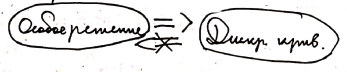
\includegraphics[width=0.4\textwidth]{int_kr.png}
	\end{figure}
\end{remark}

